\section{Introduction}
An auctioning company called ``The AuctionHouse\textsuperscript{TM}'' auctions provided goods to customers. Currently, they auction and display the goods in a warehouse just outside of city limits. Owner John wants to automate the administration of auctions and other activities using an IT solution as well as introduce some new services made possible by such a system.

\section{Expectations Summary and Conclusion}
John wants the sellers to be able to register their goods in the to-develop-system. These goods then need to be assessed and possibly removed if they lack the requirements. A couple of days before an auction, potential customers must be able to view the goods. The goods are then auctioned at location (so not through the system).\\
Currently, regular customers get mail informing them of the goods on sale, rather than having to go and see the available goods in person.\\
Payments are done through cash or card, and not through credit cards. Bigger customers get offered a special billing procedure.
The police is handed a list of goods on auctions, so they can identify any stolen goods.
Once the system is completed, a system administrator should make sure every person has the right permissions for the system, and verify that it is operating properly.

\section{Potential users and user wishes}
\subsection{Actors and Users}
What follows is a list of user (groups) that need to interact with the system directly. Also is a brief description of the wishes in customer language. This analysis is made before the analysis of the problem and design of the system, and therefore will not include any new roles that surface later on.\\
This list can also function as a dictionary for the upcoming analysis.
\begin{itemize}[noitemsep]
	\item Owner of The AuctionHouse\textsuperscript{TM} (John)\\
		The owner needs to be able to manage the staff members and their access and permissions in the system. The owner also wants to file the search requests he gets from the customers.
		The owner needs to be able to manage the staff members and their access and permissions in the system. The owner also wants to file the search requests he gets from the customers.
	\item Secretary\\
		The secretary handles some basic customer services that do not require a special role within the company. The secretary wants to register customers and sellers in the system so their credentials are saved. Currently, the secretary is also responsible for printing out the various lists that need to be distributed, like the list of items for the police. The secretary may also want to modify simple attributes of the items already in the system in case, for example, a seller wants to increase the minimum price they want for their product.
	\item Purchasing agent\\
		The purchasing agent wants to evaluate the presented goods for possible sale, and if they will be auctioned, needs to make sure they are being stored in the storehouse (which does not necessarily have to be done through the system).
	\item Private Individuals and Merchants (Owners/Sellers of the goods)\\
		Sellers need to be able to present their goods to the purchasing agent so he/she can decide whether they can be auctioned.
	\item Customers/Buyers\\
		Customers want to see the list of goods on sale, see the date they are auctioned at and potentially buy them. They also want to be able to make a request for the search of a specific item.
	\item Viewers/The public\\
		Viewers want to see the products that are going to be auctioned, and therefore need to have access to the list of goods along with their price and auctioning date(s).
	\item System Administrator\\
		The system administrator is responsible for the system's behaviour and needs to monitor system activity.
\end{itemize}

\subsection{Other Stakeholders}
Below is the list of stakeholders; people who have interests in the development of the system, or are otherwise involved with it, while not having to interface with it directly or having additional needs compared to other user groups.
\begin{itemize}[noitemsep]
	\item Regular Customer\\
		Regular customers have no extra needs or wishes. However, they are registerd in the system with their credentials and receive auction catalogues at their home address and, if they like, a list of available goods in their catagory of interest.
	\item Big Customer\\
		Big customers are essentially normal customers, but since their expenses are greater, they are offered a special billing procedure.
	\item Police\\
		The police has no need to directly access the system. However, they are offered a list (printout) of goods to follow potentially stolen goods. This list may be digitalized later in development.
\end{itemize}

\subsection{User Wishes and Stories}
Users and stakeholders need the system to be able to handle their requests. Below is a list of those wishes.
\begin{itemize}[noitemsep]
	\item Administrators: do everything below under test environments
	\item Owner: add/remove/modify/view staff members
	\item Owner: *\underline{create search request}
	\item Purchasing Agent: \underline{register}/\underline{modify} items for sale
	\item Auctioneer: mark item as sold/junk
	\item Auctioneer: \underline{delete item from the item list}
	\item Secretary: registers customers and sellers to the system
	\item Secretary: generate printouts of items for sale/sold/etc.
	\item Secretary: modify basic parameters of items (e.g. modify the auction date of an item).
	\item Secretary: \underline{register customers in the system as ``regular customers''.}
	\item Seller: view items they have for sale
	\item Seller: view items they have sold
	\item Buyer: view items they have bought
	\item Buyer: request the search for an item
	\item Public: view items that are for sale
	\item Public: view auction schedule
	\item Public: \underline{reserve books}
\end{itemize}
Legend: \underline{underlined}: User wish is made into a use case. `*': a new requirement that is introduced because of the system-to-be's existence.\\\\
To visualize this, a diagram is provided. This diagram is a ``power tree'' that shows how permissions are divided and who can do the same as another user group.
\begin{figure}[H]
	\centering
	% ignore the compilation warning, it has to do with the pdf and the graphicx package not accounting for some variable within the file, even though the variable has had no purpose for about 10 years now. #research
	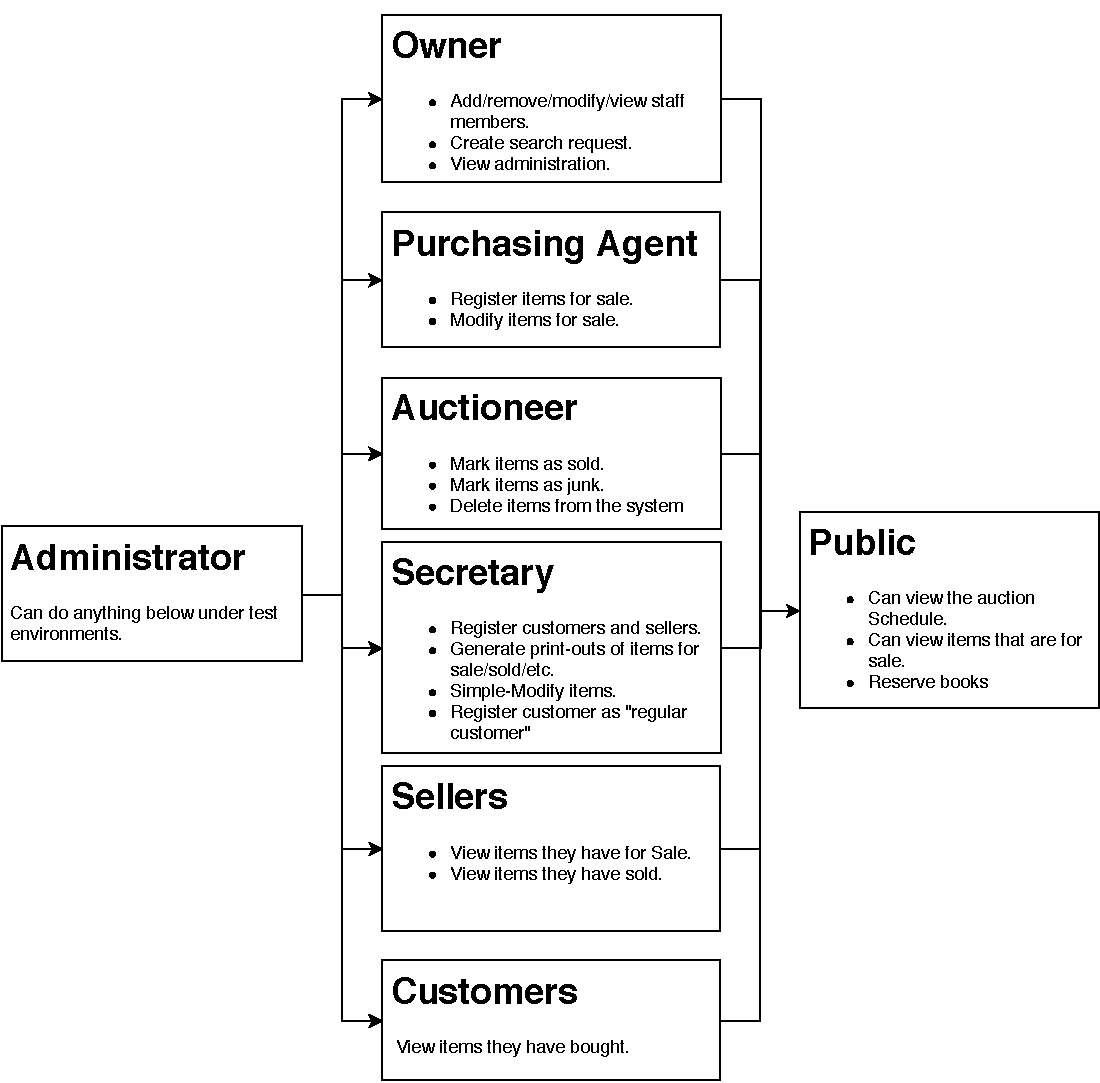
\includegraphics[scale=.75]{uml/power_tree.pdf}
	\caption*{A power tree showing the relations between user groups and permissions. Arrows indicate what permissions are inherited. For example, the Owner, Purchasing Agent, Auctioneer, etc. can all do what the public can, with some class specific permissions.}
\end{figure}